\chapter{Statistics}
\label{chapter:statistics} 
\section{Probability Distribution}
Probability distribution is a function from a set of possible outcomes of an experiment to a set of real values in the range $[0,1]$. The sum of the probabilities of occurrences of all the possible outcomes is always $1$. Now if the set of possible outcomes contains only discrete values then the function that defines the probability distribution is called probability mass function (pmf). If the set of possible outcomes contains continuous value within any range, then the function that defines the probability distribution of the experiment is called probability density function (pdf). \par \noindent There are different kinds of probability density and probability mass functions that describes the probability distribution of many natural events. Few of these probability distributions have been found to be very important in developing the statistical model of SSA. In this section those distributions along with their properties are discussed briefly
\subsection{Gamma Distribution} 
\begin{defn} \citep{gamma_distribution_book} A random variable X that is gamma-distributed with shape $k$ and scale $\theta$ is denoted by
\begin{eqnarray*}
X \sim \Gamma(k, \theta) \equiv \textrm{Gamma}(k, \theta)
\end{eqnarray*}
The probability density function using the shape-scale parametrization is
\begin{eqnarray*}
f(x;k,\theta) =  \frac{x^{k - 1}e^{-\frac{x}{\theta}}}{\theta^k\Gamma(k)} \quad \mbox{ for } x > 0 \mbox{ and } k, \theta > 0
\end{eqnarray*}
Here $\Gamma(k)$ is the gamma function evaluated at $k$.
\end{defn}
Figure \ref{fig:gamma_dist}  provides a visualization of the gamma distribution given different shape and scale parameters.
\begin{figure}[h!]
    \centering
    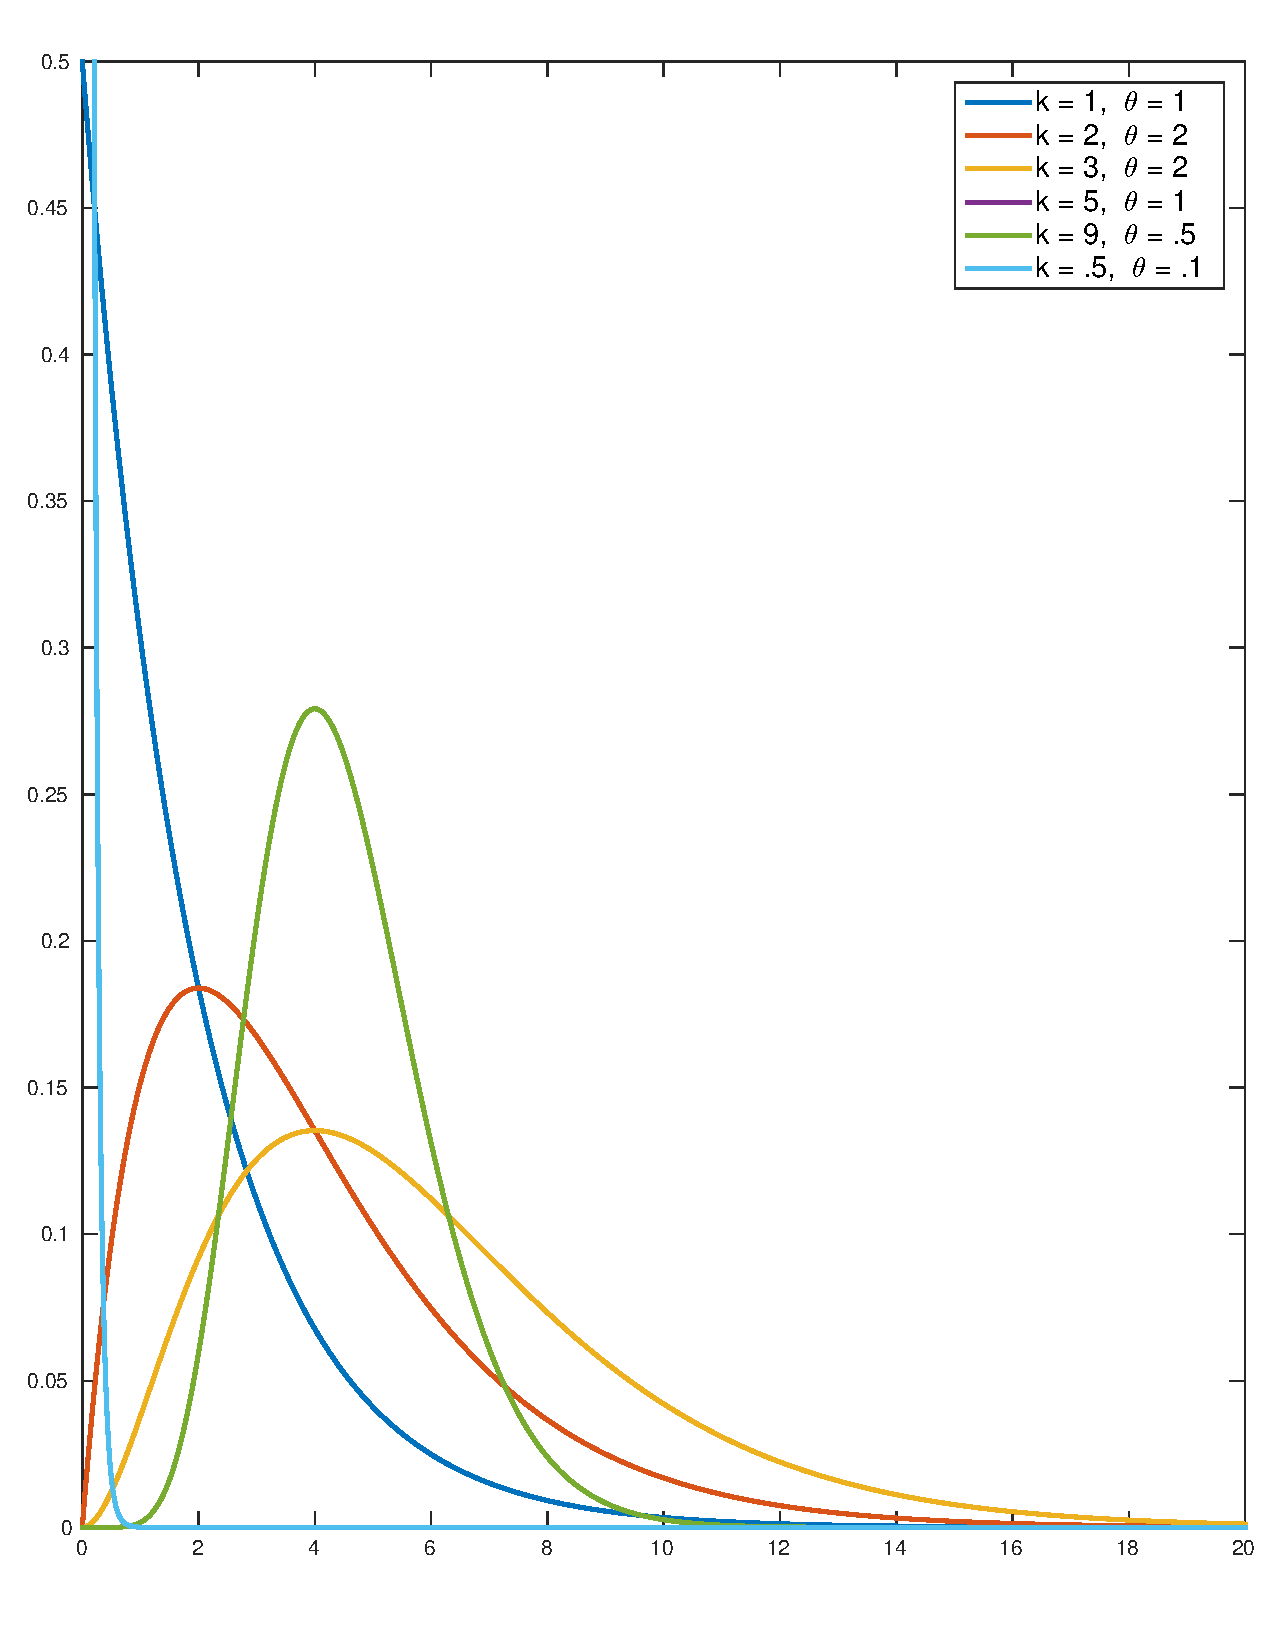
\includegraphics[width=0.9\textwidth, height=12cm]{images/GammaDistribution}
    \caption{Gamma distribution with different shape and scale parameters}
    \label{fig:gamma_dist}
\end{figure}
\subsection{Properties of Gamma Distribution}
\begin{enumerate}
\item Let $X$ be a random variable which is gamma distributed with shape parameter $k$ and scale parameter $\theta$. Then for any constant $c$, the random variable $Y = cX$ is also gamma distributed with the shape parameter $k^{'}$ and scale parameter $\theta^{'}$. Where $k^{'} = k$ and $\theta^{'} = c\theta$ \cite{scaling_of_gamma_distribution_uah}. In other words, we can write
\begin{eqnarray}
X \sim \Gamma(k,\theta) \Rightarrow cX \sim \Gamma(k,c\theta)\label{eqn:gamma_dist_property_scaling}
\end{eqnarray}
\item Le $X$ be a random variable which is gamma distributed with the shape parameter $k$ and scale parameter $\theta$. Then the mean and variance of $X$ denoted by $\mu_X$ and $\sigma^2_X$ respectively are defined as follows \citep{gamma_distribution_book}
\begin{eqnarray}
\mu_X &=& k \theta  \label{eqn:mean_gamma_dist} \\
\sigma^2_X &=& k \theta^2 \label{eqn:variance_gamma_dist}
\end{eqnarray}

\end{enumerate}
\subsection{$\chi^2$-Distribution} \citep{chi_square_definition_book} In probability theory and statistics, the chi-squared distribution (also chi-square or $\chi^2$-distribution) with $k$ degrees of freedom is the distribution of a sum of the squares of $k+1$ independent standard normal random variables. The probability density function of the chi-squared distribution is
\begin{eqnarray}
f(x;\,k) =
\begin{cases}
  \frac{x^{(k/2-1)} e^{-x/2}}{2^{k/2} \Gamma\left(\frac{k}{2}\right)},  & x \geq 0; \\ 0, & \text{otherwise}.
\end{cases}
\end{eqnarray}
where $\Gamma(k/2)$ denotes the Gamma function, which has closed-form values for integer $k$. In addition to these, the concept of central and non-central $\chi^2$-distributions, their means and variances will be useful in deriving the statistical model. Figure \ref{fig:chi-square_distribution} shows how the probability density function looks for different values of $k$
%\pagebreak
\begin{figure}[h!]
	\centering
    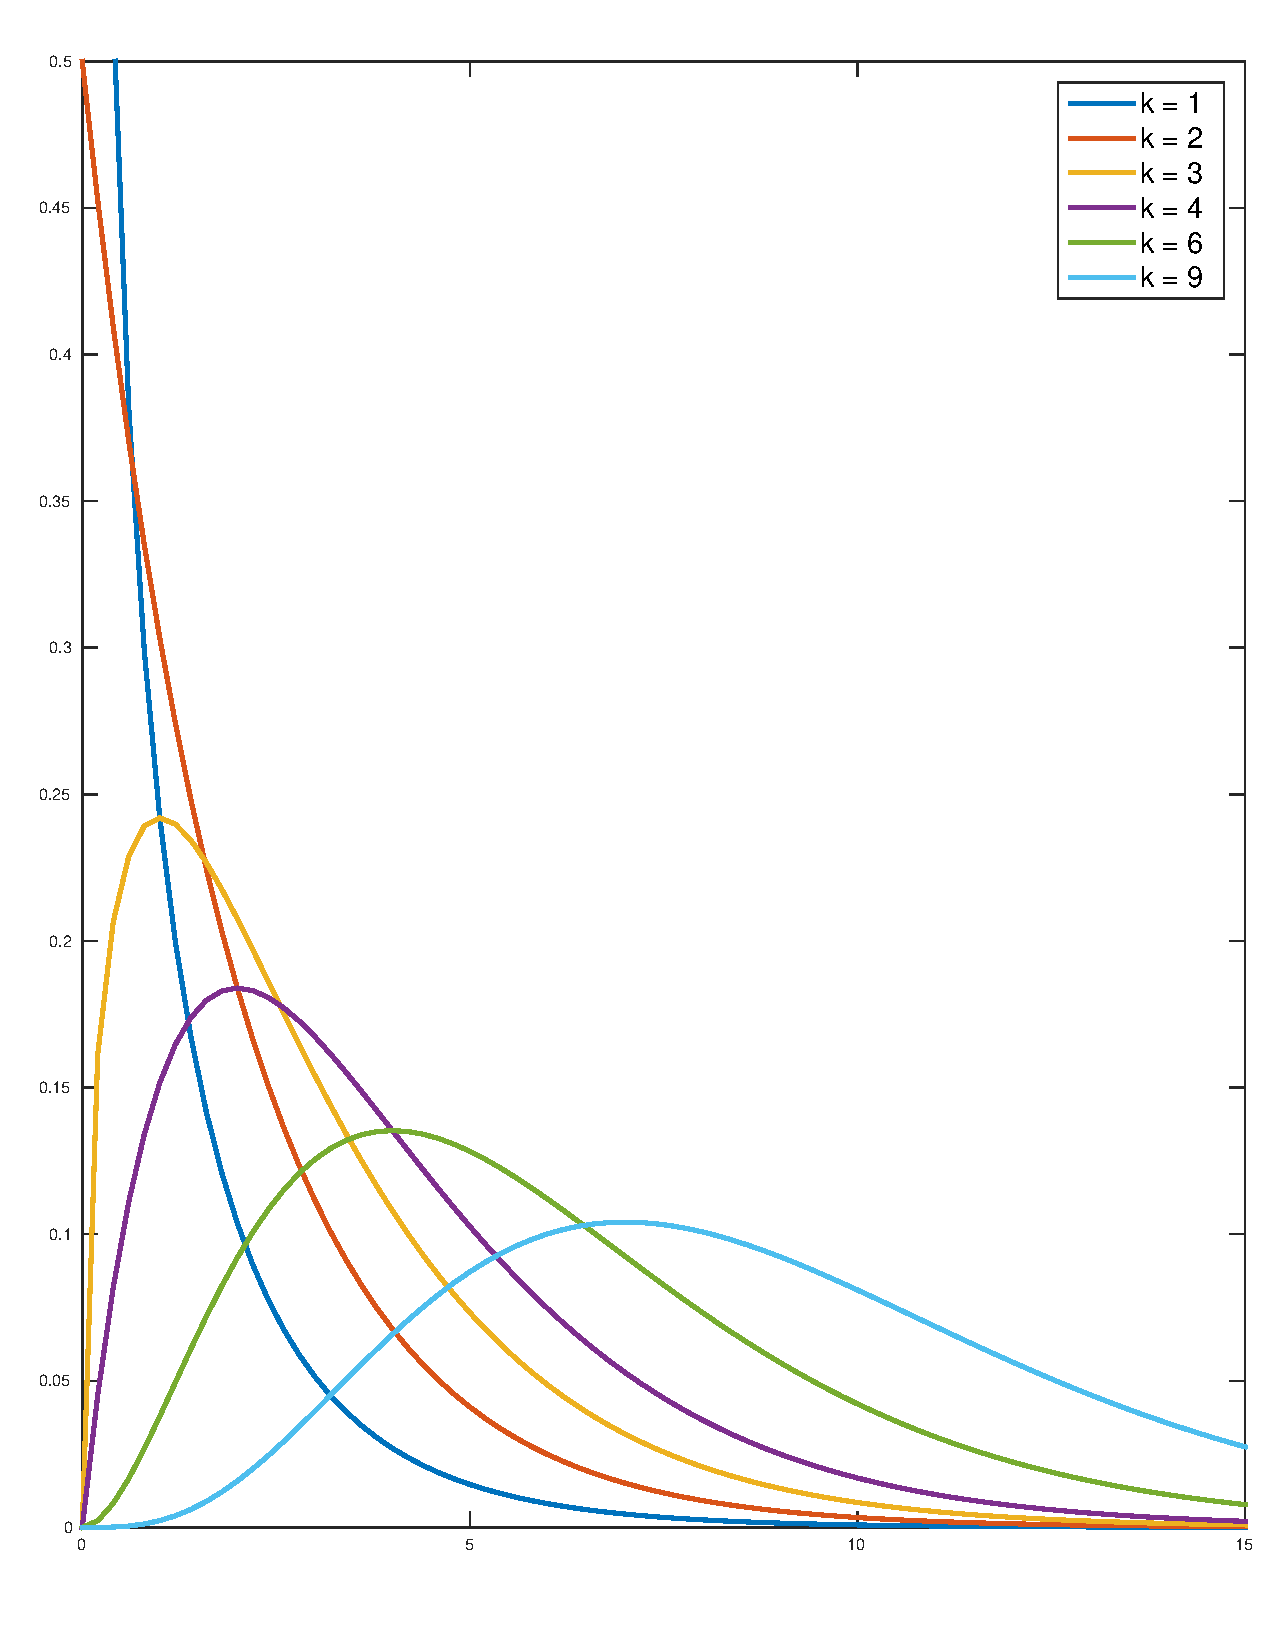
\includegraphics[width=.9\textwidth, height = 12cm]{images/ChiSquareDistribution}
    \caption{Chi-square distribution with different parameters}
    \label{fig:chi-square_distribution}
\end{figure}
\newline
\begin{defn}
\label{defn:chi_square_distribution}
\cite{distribution_cryptanalysis_kaisa_lecture_ice_break_2013} Let $X_i \sim \mathcal{N}(\mu_i,\sigma^2_i)$ where $i = 0, . . . ,k$. Then the random variable
\begin{eqnarray}
T_0 &=& \displaystyle\sum_{i=0}^{k}\frac{(X_i - \mu_i)^2}{\sigma^2_i} 
\end{eqnarray} has central $\chi^2$ distribution with $k$ degrees of freedom which is written as 
\begin{eqnarray}
T_0 &\sim & \chi^2_{k} \label{eqn:chi_square_distribution_central}
\end{eqnarray}
and the random variable 
\begin{eqnarray}
T_1 &=& \displaystyle\sum_{i=0}^{k}\frac{(X_i)^2}{\sigma^2_i} 
\end{eqnarray} has non-central $\chi^2$-distribution with $k$ degrees of freedom where the non-centrality parameter is
\begin{eqnarray}
\delta &=& \displaystyle\sum_{1=0}^{k}\frac{\mu_i^2}{\sigma_i^2} \label{eqn:chi_square_non_centrality}
\end{eqnarray} And this is written as:
\begin{eqnarray}
T_1 &\sim & \chi^2_{k}(\delta) \label{eqn:chi_square_distribution_non_central}
\end{eqnarray}
The mean and variance of the variable $T_0$ which is centrally $\chi^2$-distributed are following:
\begin{eqnarray}
\mu_{T_0} &=& k \label{eqn:chi_square_central_mean}\\
\sigma^2_{T_0} &=& 2k \label{eqn:chi_square_central_variance} 
\end{eqnarray} And the mean and variance of the variable $T_1$ which is non-centrally $\chi^2$-distributed with $\delta$ as non-central parameter is following:
\begin{eqnarray}
\mu_{T_1} &=& k + \delta \label{eqn:chi_square_non_central_mean}\\
\sigma^2_{T_1} &=& 2(k + 2\delta) \label{eqn:chi_square_central_mean}
\end{eqnarray}
\end{defn}
\subsection{Link Between $\chi^2$ and $\Gamma$ Distribution}
A $\chi^2$ variable $X$ of $k$ degrees of freedom is gamma distributed with shape $\alpha = \frac{k}{2}$ and scale $\beta=2$ \citep{chi_gamma_link_book}. That is
\begin{eqnarray}
X \sim \chi^2_{k} \Rightarrow X \sim \Gamma \left(\alpha= k/2, \beta= 2 \right) \label{eqn:link_chi_gamma}
\end{eqnarray}

%Consequently, as $nk \to \infty$, we have
% \begin{eqnarray*}
% \bar X &=& \frac{1}{n} \sum_{i=1}^{n} X_i \sim \Gamma \left(\alpha= nk/2, \beta= 2/n \right) \\
%\Rightarrow \bar X  &\sim & \mathcal{N}\left(\mu = \left(nk/2\right)\left(2/n\right), %\sigma^2 = \left(nk/2\right)\left(2/n\right)^2 \right)\\
%\Rightarrow \bar X  &\sim & \mathcal{N}\left(\mu = k, \sigma^2 = 2k/n \right) 
%\end{eqnarray*}
%So, if we set $n=1$ then for sufficiently large degree of freedom $k$ of a $\chi^2$-%distributed random variable $X$ we have
%\begin{eqnarray}
%X \sim \mathcal{N}\left(k,2k \right) \label{eqn:gamma_dist_property_normal_approximations}
%\end{eqnarray}

\subsection{Normal approximation of $\chi^2$ distribution:} \label{section:normal_approximation_of_chi_square_distribution}
\citep{chi_square_normal_approximation} For large number of degrees of freedom $k$, the chi-square distribution may be approximated by a normal distribution. Consequently we have the following two approximations.
\begin{enumerate}
\item For a sufficiently large value of $k$, a central $\chi^2$-distributed random variable $X$ with $k$ degrees of freedom is approximately normally distributed
\begin{eqnarray}
X \sim \mathcal{N}\left(k,2k \right) \label{eqn:chi_square_central_normal_approx}
\end{eqnarray}
\item For a sufficiently large value of $k$, a non-central $\chi^2$-distributed random variable $X$ with $k$ degrees of freedom and $\delta$ as non-centrality parameter is approximately normally distributed
\begin{eqnarray}
X \sim \mathcal{N}\left(k+\delta,2 \left(k+ 2\delta \right) \right) \label{eqn:chi_square_non_central_normal_approx}
\end{eqnarray}
\end{enumerate}


\subsection{Normal approximation of $\Gamma$ Distribution} \label{section:link_gamma_normal_distribution}
Let the shape and scale parameters of a gamma distribution be $\alpha$ and $\beta$. Asymptotically, given that for a shape parameter $\alpha$,  going to infinity, a gamma distribution converges towards a normal distribution with expectation  $\mu = \alpha\cdot \beta$ and variance  $\sigma^2 = \alpha\, \beta^2$ \cite{normal_approximation_of_gamma_distribution_uah}.

\subsection{Binomial Distribution}
As defined in \cite{binomial_distribution_defn}, the binomial distribution with parameters $n$ and $\theta$ is the discrete probability distribution of the number of successes in a sequence of $n$ independent ``$yes/no$'' experiments, each of which yields success with probability $\theta$. The probability of getting exactly $k$ successes in $n$ trials is given by the probability mass function
\begin{eqnarray}
f(k;n,\theta) = \Pr(X = k) = {n\choose k}\theta^k(1-\theta)^{n-k} \label{eqn:binomail_distribution_pmf}
\end{eqnarray}
for $k = 0, 1, 2, ..., n$, where ${n\choose k}=\frac{n!}{k!(n-k)!}$ is the binomial coefficient, hence the name of the distribution. \par \noindent Let $N$ be the number of data (sample size), $M$ be the number of cells with different probabilities $p(\eta), \eta = 1, 2, . . . , M$. Now if $\omega(\eta)$ denotes the number of data in cell $\eta$, then
$\omega(\eta) \sim \mathcal{B}(p(\eta))$. As mentioned in \cite{distribution_cryptanalysis_kaisa_lecture_ice_break_2013}, for large $N$ we have 
\begin{eqnarray}
\omega(\eta) \sim \mathcal{N}(Np(\eta), Np(\eta)) \approx \mathcal{N}(Np(\eta), N/M) \label{eqn:binomial_distribution_normal_approximation}
\end{eqnarray}

\section{Capacity}
\subsection{Capacity of a Distribution} \label{section:capacity_of_a_distribution}
Given a function $f:X \rightarrow Y$, $x \in X$, $\eta \in Y$, and $X$ is uniformly distributed, the probability of $f(x) =\eta$ is denoted by $p_{\eta}$ defined as 
\begin{eqnarray}
p_{\eta} = |X|^{-1}\#\lbrace x \in X \;|\; f(x) = \eta \rbrace \label{eqn:p_eta_a}
\end{eqnarray}  
The probability distribution of the function $f$ is described by the pmf $p = (p_{\eta})$. The uniformity of a distribution $p$ is measured by its capacity, also called as Squared Euclidean Imbalance. Capacity of a distribution is computed from its squared distance from the uniform distribution. If the capacity of a distribution $p$ is denoted by $C_p$, then it can be formally written as 
\begin{eqnarray}
C_{p} = |Y|\displaystyle\sum_{\eta \in Y}(p_{\eta} - |Y|^{-1})^2 \label{eqn:capacity_of_a_distribution}
\end{eqnarray}Let $p(a) = (p_{\eta}(a))$ denote a probability distribution over domain $Y$ in a family of distributions parametrized by $a \in I$. We consider $a$ as a uniformly distributed random variable. We assume that this family of probability distributions satisfies the following hypothesis. 
\begin{hyp}\label{hyp:hypothesis_on_p_eta_a}
For each fixed $\eta \in Y$, the probability $p_{\eta}(a)$ is a random variable and independently distributed and follow the normal distribution
\begin{eqnarray*}
p_{\eta}(a) \sim \mathcal{N}\left(\mu,\sigma^2\right) 
\end{eqnarray*}
where $\mu = |Y|^{-1}$
\end{hyp}For an arbitrarily fixed $a$, the capacity of $p(a) = \left(p_{\eta}\left(a\right)\right)$ is denoted by $C(a)$. Then
\begin{eqnarray}
C\left(a\right) = |Y|\displaystyle\sum_{\eta \in Y}(p_{n}\left(a\right) - |Y|^{-1})^2 \label{eqn:defn_c(a)}
\end{eqnarray}
The average capacity over the parametrized probability distributions $p(a)$ is defined by 
\begin{eqnarray}
C = |I|^{-1}\displaystyle\sum_{a \in I}C(a) \label{eqn:average of C a}
\end{eqnarray}
\subsection{Distribution of Capacity}
\begin{theorem}\label{general capacity distribution}
Given a family $p(a), a \in I$ of probability distributions that satisfies Hypothesis 1, the capacity $C(a)$ is gamma distributed $$C(a) \sim \Gamma\left(\frac{|Y|-1}{2},\frac{2C}{|Y|-1}\right)$$ with mean $C$ and variance $\frac{2C^2}{|Y|-1}$
\end{theorem}
\begin{proof}
Let $\mu_{C(a)}$ and $\sigma^{2}_{C(a)}$ denote the mean and variance of $C(a)$ respectively. According to (\ref{eqn:average of C a}) we have $\mu_{C(a)} = C$. Let us now examine the parametrized statistic $Q(a)$ defined as
\begin{eqnarray}
Q(a) &=& \displaystyle\sum_{\eta}\frac{\left(p_{\eta}(a) - \mu_{p_{\eta}(a)}\right)^2}{\sigma^{2}_{p_{\eta}(a)}} 
\end{eqnarray}
From Hypothesis \ref{hyp:hypothesis_on_p_eta_a}, we know that $p_{\eta}(a)$ is identically and independently normally distributed. As a result, using Hypothesis \ref{hyp:hypothesis_on_p_eta_a} and Definition  \ref{defn:chi_square_distribution}, we can write
\begin{eqnarray}
Q\left(a\right) &=& \displaystyle\sum_{\eta}\frac{(p_{\eta}(a) - |Y|^{-1})^2}{\sigma^{2}} \sim  \chi^2_{|Y|-1} \label{eqn:Q(a)}
\end{eqnarray}
Let us multiply both sides of (\ref{eqn:Q(a)}) by the cardinality of the set $Y$ and variance of the distribution $p_{\eta}(a)$.  The result is following:
\begin{eqnarray}
|Y|Q(a)\sigma^{2} &=& |Y|\displaystyle\sum_{\eta}\left(p_{\eta}(a) - |Y|^{-1}\right)^2 \label{eqn:Y_Q_sigma}
\end{eqnarray}
As per definition of capacity of a distribution given in (\ref{eqn:capacity_of_a_distribution}), the right hand side of (\ref{eqn:Y_Q_sigma}) is the capacity of the distribution $p(a)$, which can be denoted as $C(a)$ as per our convention. So, we get
\begin{eqnarray*}
C(a) &=& |Y|\sigma^{2}Q(a)
\end{eqnarray*}
Now if we plug (\ref{eqn:Q(a)}) in (\ref{eqn:link_chi_gamma}), then we can write 
\begin{eqnarray}
Q(a) &\sim& \Gamma\left(\frac{|Y-1|}{2},2\right) \label{eqn:Q_gamma_distributed}
\end{eqnarray}
We see $|Y|$ is a constant and as per Hypothesis \ref{hyp:hypothesis_on_p_eta_a}, $\sigma^2$ is also a constant. According to (\ref{eqn:Q_gamma_distributed}), $Q(a)$ is gamma distributed. So, as per the property of gamma distribution given in (\ref{eqn:gamma_dist_property_scaling}), we can write 
\begin{eqnarray} 
C(a) &\sim & \Gamma\left(\frac{|Y-1|}{2},2|Y|\sigma^{2}\right) \label{eqn:distribution_of_C_a}
\end{eqnarray}
Let us denote the mean of $C(a)$ over all $a \in I$ by $C$. As per the property of gamma distribution given in (\ref{eqn:mean_gamma_dist}) the mean of the gamma distributed random variable is the multiplication of its shape and scale parameter. Consequently, from (\ref{eqn:distribution_of_C_a}), the mean  $C$ is as follows
\begin{eqnarray*}
C &=& |Y-1||Y|\sigma^2\\
\end{eqnarray*} Which implies that
\begin{eqnarray}
\sigma^2 &=& \frac{C}{|Y-1||Y|} \label{eqn:variance_of_p_eta_i}
\end{eqnarray} 
Now by plugging the $\sigma^2$ from (\ref{eqn:variance_of_p_eta_i}) in (\ref{eqn:distribution_of_C_a}), we obtain the following result 
\begin{eqnarray}
C(a) \sim \Gamma\left(\frac{|Y|-1}{2},\frac{2C}{|Y|-1}\right) \label{eqn:distribution_of_C a_second}
\end{eqnarray}
The first claim of the theorem is now proven and it remains to show that the variance is $\sigma^2_{C(a)} = \frac{2C^2}{Y-1}$. As per the property of gamma distribution given in (\ref{eqn:variance_gamma_dist}), variance of a gamma distributed variable  is the multiplication of it's shape parameter and the square of scale parameter. Using this property in (\ref{eqn:distribution_of_C a_second}), we find the variance $\sigma^2_{C(a)}$ as follows 
\begin{eqnarray*}
\sigma^{2}_{C(a)} &=& \frac{|Y-1|}{2}\left(\frac{2C}{|Y-1|}\right)^2 \\ 
&=& \frac{2C^2}{|Y|-1}
\end{eqnarray*}
\end{proof}

\section{A statistical test to distinguish distribution} \label{section:statistical_test} In the applications of cryptanalysis, the task is to distinguish between cipher and random behavior based on an observed distribution computed from sample data. Now we present a statistical test to accomplish this task. To perform the statistical test, we are in need of a statistic computed from the cipher data distribtuion. We denote this statistic as $T$. For the statistical test we are presenting here, it is essential for $T$ to be defined in a way that it is normally distributed. Suppose we already know two normal deviates $T_0$ and $T_1$ such that
\begin{eqnarray*}
T_0 \sim \mathcal{N}\left(\mu_{T_0},\sigma^{2}_{T_0} \right)\\
T_1 \sim \mathcal{N}\left(\mu_{T_1},\sigma^{2}_{T_1} \right)
\end{eqnarray*} and assuming without loss of generality that $\mu_{T_0} < \mu_{T_1}$. Given a $T$ computed from a sample about which we know that it follows either the distribution of $T_0$ or $T_1$. The task is to decide which of those two it is. The test is defined by a value $\tau$. If $T\leq \tau$ the outcome of the test is that $T$ is drawn from the distribution of $T_0$ and if $T > \tau$ then $T$ is drawn from the distribution $T_1$. The error probabilities are defined as 
\begin{eqnarray*}
\alpha_0 &=& \Pr\left(T_0\;|\;T > \tau\right)\\
\alpha_1 &=& \Pr\left(T_1\;|\;T \leq \tau \right)
\end{eqnarray*}
That is, $\alpha_0$ is the probability that the test outputs $T_1$ when the reality is $T_0$. Similarly $\alpha_1$ is the probablity that the test outputs $T_0$ when the reality is $T_1$. To make the error probabilities less than $\alpha_0$ and $\alpha_1$, we must select $\tau$ to satisfy
\begin{eqnarray}
\mu_{T_0} + \sigma_{T_0}\zeta_0 \leq \tau \leq \mu_{T_1} - \sigma_{T_1}\zeta_1 \label{eqn:selecting_tau_range}
\end{eqnarray} where $\mathit{\Phi}(\zeta_i) = 1 - \alpha_i$ for $i \in \mathbb{Z}_2$ for the cumulative distribution function $\mathit{\Phi}$ of the standard normal distribution. That is, $\zeta_i$ indicates how many standard deviation beyond the mean is required to bound the probability of wrongly choosing $T_{i-1}$ by at most $\alpha_i$. The Figure \ref{fig:single_tau_range} shows the range of feasible values of $\tau$. In Figure \ref{fig:single_tau} shows how to choose a single value of $\tau$. Note that in Figure \ref{fig:single_tau}, the area on the right side of the yellow line under the red curve indicates $\alpha_0$ and the area on the left side of the yellow line under the blue curve indicates $\alpha_1$
\begin{figure}[h!]
    \centering
    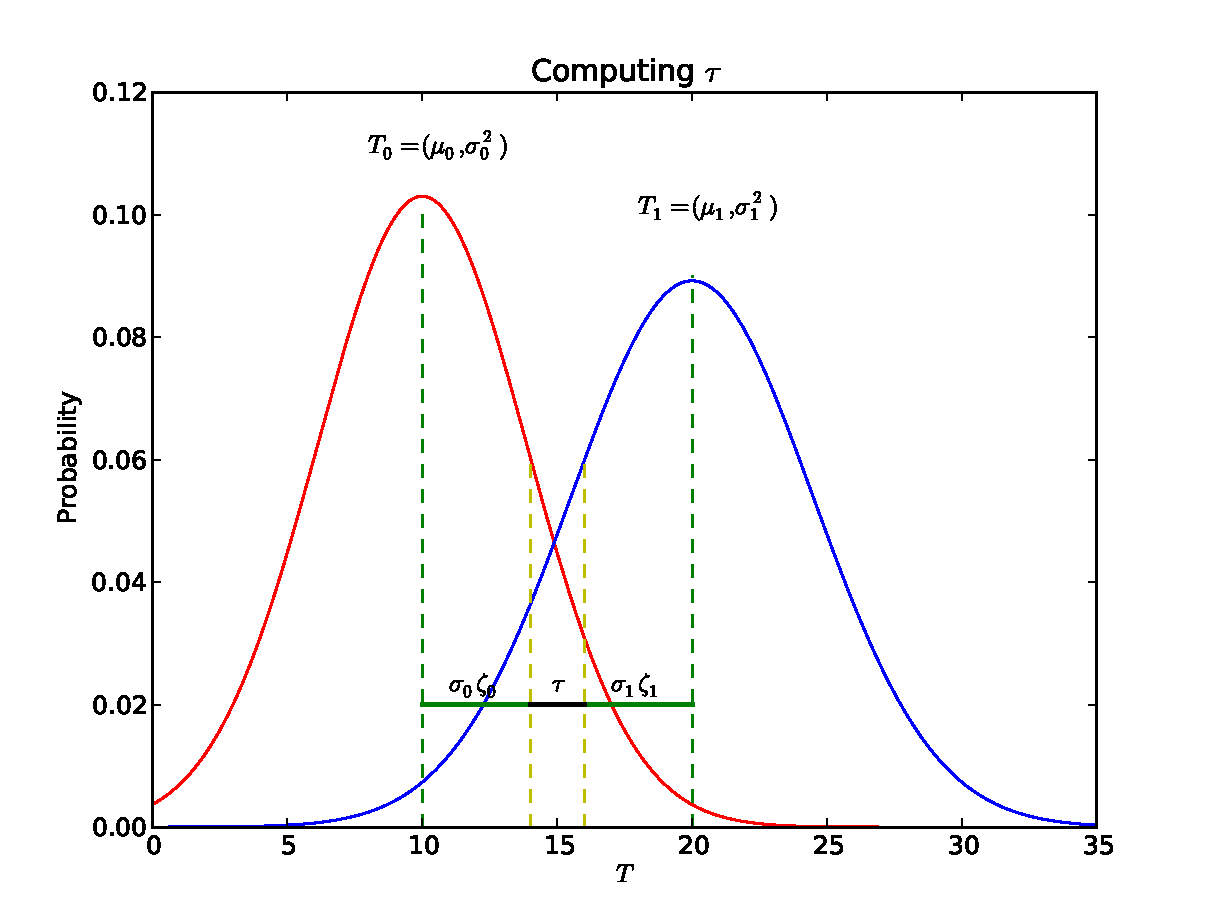
\includegraphics[width=\textwidth , height = 8cm]{images/feasible_range_of_tau}
    \caption{Choosing a range of feasible values of $\tau$}
    \label{fig:single_tau_range}
\end{figure}
In the applications of cryptanalysis the distribution of $T_1$ is determined by the cipher while $T_0$ represents random behaviour. If the cipher distribution has non-zero capacity the statistic $T$ given above can be used. The parameters of $T_1$ depend on the number $N$ of plaintexts, while the parameters of $T_0$ are constant with $N$ as the distribution is uniform and its capacity is equal to zero. Then the distributions of $T_0$ and $T_1$ move apart as $N$ grows. The phenomenon is presented in Figure \ref{fig:single_tau_as_distributions_distinguishes}. In this figure, the blue line has moved on the right along the $X$-axis, which has made the error areas smaller. Then the above equation allows to determine the sample size $N$ which is sufficient to find a threshold $\tau$ that gives a test with as small non-zero error probabilities $\alpha_0$ and $\alpha_1$ as desired.
\begin{figure}[h!]
    \centering
    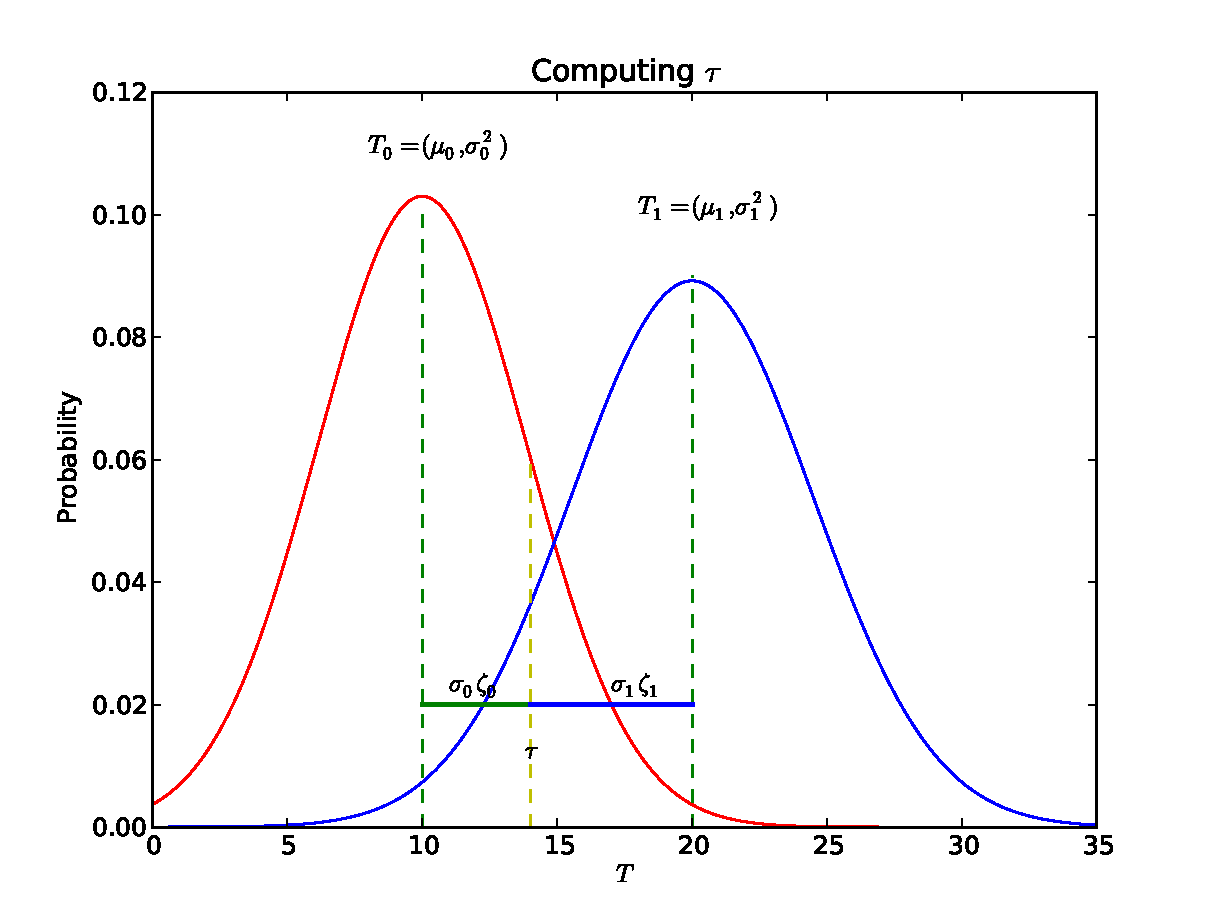
\includegraphics[width=\textwidth , height = 8cm]{images/single_tau}
    \caption{Choosing a single value of $\tau$. That is $\mu_0+\sigma_0\zeta_0 = \mu_1 - \sigma_1\zeta_1$}
    \label{fig:single_tau}
\end{figure}
\begin{figure}[h!]
    \centering
    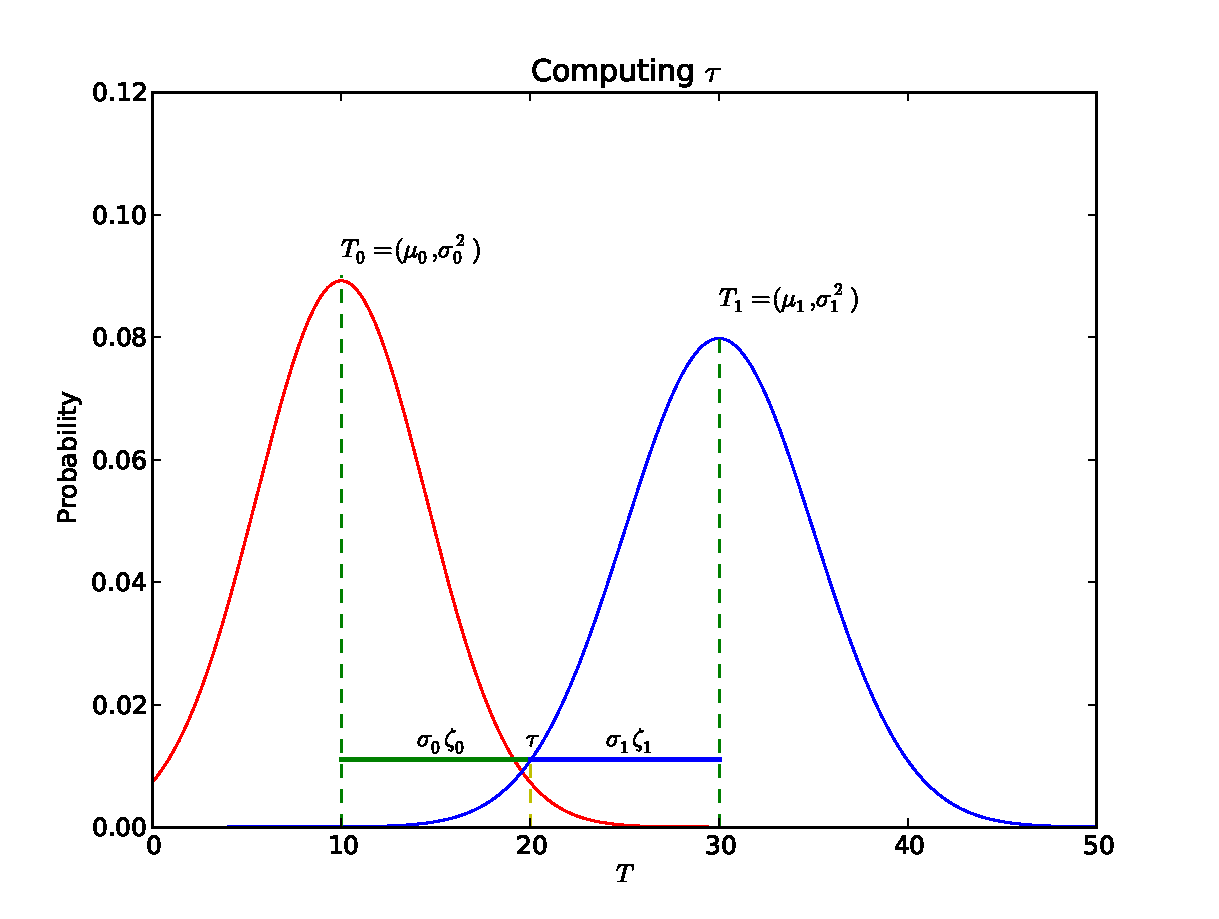
\includegraphics[width=\textwidth , height = 8cm]{images/single_tau_as_the_distributions_distinguishes}
    \caption{As $T_0,T_1$ move apart, $\tau$ can be chosen for smaller error rate}
    \label{fig:single_tau_as_distributions_distinguishes}
\end{figure}
\par \noindent In Section \ref{section:statistic_T}, we have defined statistic $T$ which we have used to develop the statistical model in the Chapter \ref{chapter:statistical_distinguishers}.

\section{Statistic $T$ for the statistical test} \label{section:statistic_T}
We already have mentioned that statistic $T$ is computed from cipher data distribution. Note that the cipher data is computed from a set of chosen plaintexts. Let us call this set of chosen plaintexts as sample denoted by $\phi$. Let us consider a fuction $\Omega:\phi \rightarrow Y$ derived from the encryption function. Let $\omega:Y \rightarrow \mathbb{Z}$ another function such that $\omega\left(\eta \right)$ is the number of times a value $\eta \in Y$ is observed as the output of function $\Omega$, that is
\begin{eqnarray*}
\omega\left( \eta \right) = \# \left\lbrace x \in \phi \; \vert \; \Omega \left( x \right) = \eta \right\rbrace , \eta \in Y
\end{eqnarray*}
Now given a sample $\phi$ of size $N$, we define $T$ as following:
\begin{eqnarray*}
T&=&\displaystyle\sum_{\eta \in Y}\frac{\left( \omega(\eta) - N|Y|^{-1}\right)^2}{N|Y|^{-1}} \\ 
\end{eqnarray*} In sections \ref{section:sampling_with_replacement} and \ref{section:sampling_without_replacement}, we have discussed how the statistic $T$ is distributed when the sample $\phi$ is sampled with or without replacement. 

\subsection{Sampling with replacement} \label{section:sampling_with_replacement} Let $p_{\eta}$ denote the expected probability of getting $\Omega(x) = \eta$ when $N=1$. We also observe that that $\omega({\eta})$ is binomially distributed. As per property of binomial distribution given in (\ref{eqn:binomial_distribution_normal_approximation}) we can write 
\begin{eqnarray}
\mu_{\omega({\eta})} = Np_{\eta} \\
\sigma^2_{\omega({\eta})} = N|Y|^{-1}
\end{eqnarray}
Now, according to the definition of $\chi^2$-distribution given in (\ref{eqn:chi_square_distribution_non_central}), the statistic
\begin{eqnarray*}
T&=&\displaystyle\sum_{\eta \in Y}\frac{\left( \omega(\eta) - N|Y|^{-1}\right)^2}{N|Y|^{-1}} \\ 
&=& \displaystyle\sum_{\eta \in Y}\frac{\left( \omega(\eta) - N|Y|^{-1}\right)^2}{\sigma^2_{\omega({\eta})}}\\
&=& \displaystyle\sum_{\eta \in Y}\frac{\left( \omega(\eta) - N|Y|^{-1}\right)^2}{\sigma^2_{\omega({\eta})- N|Y|^{-1}}}
\end{eqnarray*}
is non-centrally $\chi^2_{|Y|-1}(\delta)$-distributed. To calculate the the non-central parameter $\delta$, we need to know the mean and variance of $\omega(\eta) - N|Y|^{-1}$. Observe that $N|Y|^{-1}$ is a constant and the mean of $\omega(\eta)$ is $Np_{\eta}$. Consequently the mean of $\omega(\eta) - N|Y|^{-1}$ is $Np_{\eta} -N|Y|^{-1}$. And variance of $\omega(\eta)$ and $\omega(\eta) - N|Y|^{-1}$ are same. As a result we can calculate $\delta$ as following
\begin{eqnarray*}
\delta &=& \displaystyle\sum_{\eta \in Y} \frac{\left(Np_{\eta} -N|Y|^{-1} \right)^2}{\sigma^2_{\omega({\eta})- N|Y|^{-1}}}\\
&=& \displaystyle\sum_{\eta \in Y} \frac{N^2\left(p_{\eta} -|Y|^{-1} \right)^2}{N|Y|^{-1}}\\
&=& N \displaystyle\sum_{\eta \in Y} \frac{\left(p_{\eta} -|Y|^{-1} \right)^2}{|Y|^{-1}} \\
&=& NC 
\end{eqnarray*}Where $C$ is the capacity of the distribution $p=(p_{\eta})$. Now according to Definition \ref{defn:chi_square_distribution}, the mean and variance of $T$, denote by $\mu_T$ and $\sigma^2_T$ are 
\begin{eqnarray*}
\mu_T &=& |Y| - 1 + NC\\
\sigma^2_T &=& 2\left(|Y| -1 + 2NC\right) 
\end{eqnarray*}According to the normal approximation of $\chi^2$-distribution as mentioned in Section \ref{section:normal_approximation_of_chi_square_distribution} we can write 
\begin{eqnarray}
T &\sim & \mathcal{N} \left( |Y| - 1 + NC, 2\left(|Y| -1 + 2NC\right) \right)
\end{eqnarray}

\subsection{Sampling without replacement} \label{section:sampling_without_replacement}
When $\phi$ is sampled without replacement, the number of different possible samples decreases as the size of the samples increases. The difference between those different samples also decreases as the size of the samples increases. Which implies, as the sample size grows, the value of $T$ also differs small for different samples. As a result, the variance of $T$ decreases. This is indeed, because when we consider the maximum sample size, there is only one possible sample and only one possible value of $T$ resulted from this sample. Which means, in this case $T$ has zero variance. This phenomenon has been taken into account by Blondeau and Nyberg in \citep{sample_without_replacement}. They have introduced a co-efficient $B$ in the computation of the mean and variance of $T$ using sample without replacement. When the sample size is small, $B$ is almost one and as the sample size grows towards the maximum size, $B$ approaches to zero and becomes zero when the sample size is maximum. \par \noindent According to \citep{sample_without_replacement}, we can define $B$ as $\left(1 - \frac{N}{\lvert \phi \rvert_{max}} \right)$. Here $\lvert \phi \rvert_{max}$ is the largest possible size of a valid sample $\phi$. And the mean and variance of $T$ are following:
\begin{eqnarray}
\mu_T &=& \left(\lvert Y \rvert - 1\right)B + NC \\
\sigma^2_T &=& 2\left(\lvert Y \rvert - 1\right)B^2 + 4BNC
\end{eqnarray} \par \noindent In the next chapter we have extended this discussion of $T$ considering the associated trail of the attack. That is, we have defined the function $\Omega$ considering the the encryption function and the SS trail. However, we will only focus on the case of sampling with replacement in the rest of the thesis. Sampling with replacement is already good enough, in real life cryptanalysis. As shown in \citep{sample_without_replacement}, the method of sampling without replacement offers some advantage when the sample size is close to the full codebook. In an upcoming paper \citep{kaisa_mohsin_2015} the statistical model developed in this work has been extended to the case of sampling without replacement.